\documentclass{article}

\usepackage[utf8]{inputenc}
\usepackage[T1]{fontenc}
\usepackage[french]{babel}

\usepackage{caption}
%\usepackage{pgfplots}
\usepackage{listings}
\usepackage{graphicx}
\usepackage{footnote}
\usepackage{amsmath}
\usepackage{amsthm}
\usepackage{graphicx}
\usepackage{url}
\usepackage{amssymb}
\usepackage{mathrsfs}
\usepackage{multirow}
\usepackage{amsfonts}
\usepackage[boxed,linesnumbered,noend]{algorithm2e}
\usepackage{qcircuit}
\usepackage{enumerate}
\usepackage{eurosym}

\newtheorem{thm}{Theorem}
\newtheorem{prop}{Propriety}
\newtheorem{lemma}{Lemma}
\newtheorem{defi}{Definition}
\newtheorem{coro}{Corollary}



\setlength{\oddsidemargin}{0pt}
% Marge gauche sur pages impaires
\setlength{\evensidemargin}{0pt}
% Marge gauche sur pages paires
\setlength{\textwidth}{470pt}
% Largeur de la zone de texte 
\setlength{\topmargin}{0pt}
% Pas de marge en haut
\setlength{\headheight}{13pt}
% Haut de page
\setlength{\headsep}{10pt}
% Entre le haut de page et le texte
\setlength{\footskip}{40pt}
% Bas de page + séparation
\setlength{\textheight}{630pt}
% Hauteur de la zone de texte

\title{Programmation Avancée des Architecture Multicoeurs}
\author{Gaël Thomas\\
\url{gael.thomas@telecom-sudparis.eu}\\
\url{http://www-inf.telecom-sudparis.eu/COURS/chps/paam/}}
\date{}

\newcommand{\note}{\medskip\noindent\underline}

\begin{document}
\maketitle
\tableofcontents
\newpage


Technique d'optimisation bas niveau (ASM) sur des architectures de "petits multicolores" (environ 30 cœurs). Pas d'OpenMP, pas de MPI (trop haut niveau).

\paragraph{Référence} \emph{The Art of parallel programming}, M.Herlihy, N.Shavit (Bible, à acheter !)

\paragraph{Attention} Les transparents n'ont pas été modifiés depuis 7 ans : ne pas trop s'y fier (50\% d'information données ne sont plus dans les slides en fait).

\section{Introduction}
Depuis une dizaine d'année, les appareils informatiques ont complètement changé (tour moche en plastiques...). D'un côté l'informatique embarqué (téléphones, voitures, trains, ...) s'est développée, avec peu de ressources de calcul $\to$ modèle du \emph{mainframe} : serveur/terminaux. Les centres de données sont désormais propulsé par des architectures multicoeurs (le dégagement thermique augmente avec le carré de la fréquence, on augmente donc le nombre de coeurs car l'augmentation est linéaire avec la consommation). La loi de Moore restant toujours possible (miniaturisation des transistors), on intègre des clusters de machine complet sur un die.

De nos jours, pour gagner des performances, il faut augmenter le parallélisme, ce qui est difficile. Nous allons bien entendu travailler dessus, ainsi que sur le placement (caches).

On a un aspect de plus en plus nomade de l'informatique (on masque la localisation : possibilité de continuer un travail sur plusieurs machine), rendu possible par la centralisation des calcul. La technique utilisée est la \emph{virtualisation}, ce qui est également possible pour le HPC. On n'utilise quasiment plus la machine telle qu'elle est. L'idée est d'utiliser une "machine dans une machine", ce qui introduit une \emph{couche de virtualisation} qui modifie les comportement (il s'agit du sujet de recherche de notre professeur).

\paragraph{Plan}
\begin{enumerate}[I]
\item Etude des multicoeurs (NUMA) $\to$ TP très sympa pour mesurer la latence mémoire
\item Concurrence en mémoire partagée
\item Algorithme classique et sans verrous
\item Mémoire transactionnelle
\end{enumerate}


\subsubsection*{Rappel sur les verrous (mutex)}
Les threads lisent et écrivent des valeurs dans un \emph{registre} en mémoire, par exemple une base de donnée d'une banque lue et écrit par des distributeurs. Certains registres sont en lecture, lecture/écriture, écriture. On s'intéresse ici aux registres en lecture/écriture.

Le problème réside dans le fait qu'il est possile d'avoir des accès \emph{concurrents} qui mènent à des données \emph{incohérentes} (du point de vue du programmeur !). C'est le problème du \emph{chat-mouton} (essayer de dessiner un chat et un mouton sur le même tableau par deux enfants, ça ne va pas trop marcher...).

\paragraph{Problème classique des bases de données sur lequel est basé tout le cours :} Les comptes en banque. Un processus $p_1$ lit le compte et le met à jour en ajoutant deux euros. Un ami, processus $p_2$ est avec votre carte bleue et débite 100\euro (lire le compte puis le met à jour). Il est possible de miraculeusement gagner 100\euro : 
\begin{itemize}
\item[$p_1$ :] $a$ lit le contenu ($cpt=100$\euro)
\item[$p_1$ :] ajoute 2 à $a$ ($cpt=100$\euro, $a=102$\euro)
\item[$p_2$ :] $b$ lit le compte ($cpt=100$\euro)
\item[$p_2$ :] retirer 100 à $b$ ($cpt=100$\euro)
\item[$p_2$ :] $b$ devient le nouveau solde ($cpt=0$\euro)
\item[$p_1$ :] $a$ devient le nouveau solde ($cpt=102$\euro)
\end{itemize}
\bigskip

Le retrait a disparu ! Pour palier à ce fait, on utilise un verrou pour retirer l'accès concurrent. Les régions dangereuses sont appelées \emph{sections critiques} et doivent être exécutés \emph{atomiquement}. Le verrou joue le rôle de feu de signalisation pour les programmes : tant que le verrou n'est pas libre j'attends, si il est là je le prends et je suis le seul à pouvoir le prendre.

On entoure les section critiques par le verrou:
\begin{algorithm}
lock(mutex) \tcp*{bloquant si jamais le mutex n'est pas disponible}
\tcc{section critique 1\;
Par exemple ajouter 2\euro\;}
unlock(mutex)\;
\end{algorithm}

\begin{algorithm}
lock(mutex) \tcp*{bloquant si jamais le mutex n'est pas disponible}
\tcc{section critique 2\;
Par exemple retirer 100\euro\;}
unlock(mutex)\;
\end{algorithm}

\paragraph{Attention aux situations de famines !} Il ne faut pas qu'une suite d'opérations menant à un interbloquage des threads soit possible ! Il faut éviter d'inverser l'ordre des verrous (dans la doc Linux par exemple, il est indiqué dans quel sens prendre les verrous !).


\paragraph{Petit aparté} Attention, cela revient rapidement costaud niveau math derrière, le parti pris ici est de retirer le maximum de la théorie pour passer au code.

\paragraph{Notation} Un exam final sur 100\% et un devoir surprise à un moment sur 10\%. Une annale sont disponibles sur le site (attention, ne pas se fier à la difficulté car elle dépend de la promo).

\paragraph{Conseil} Garder un œil sur les revues scientifique, même si vous vous destinez à un parcours d'ingénieur (grrrr...).


\section{Multicoeurs}
Idée : comprendre au niveau matériel et pourquoi certains comportement au niveau logiciel peuvent sembler étranges.

\emph{Auparavant} Loi de Moore : la densité d'intégration des transistors double tout les 18 mois. Cette puissance permettait d'augmenter la fréquence, qui s'est heurtée à la dissipation thermique (la consommation augmente avec le carré de la fréquence). On sait par contre que ça ne sera pas toujours le cas : les interconnexions entre coeurs peuvent également tirer beaucoup d'énergie, bien que ce ne soit pas le facteur limitant de nos jours.

De nos jours, il est possible de louer des serveurs vers 80 cœurs par Amazon : c'est le \emph{cloud computing}.
\bigskip

\paragraph{Premier grand problème:}
Il faut paralléliser le code ! Et ce n'est pas suffisant.
\bigskip

Au niveau architecturale, il est impossible d'utiliser une topologie classique à base de bus, car environ une instruction sur quatre est un accès mémoire. Pour palier à cela, on change la topologie : \emph{diviser pour mieux régner}. On utilise un bus pour relier plusieurs cœurs entre eux et former une \emph{nœuds} de calcul, puis on les relies entre eux.
\bigskip

\paragraph{Terminologie}
\begin{itemize}
\item[Unité de calcul :] capable de faire des additions/opération (on appelait cela processeur auparavant
\item[Unité mémoire :] Contrôleur permettant la traduction adressage virtuelle/physique
\item[Contrôleur d'interruption :] Gère les interruptions (principalement par les périphériques
\item[Un timer :] Indépendant par cœur (imaginez si une seule horloge à 800 kHz devait communiquer chaque tick au 50 cœurs...). Lors de l'utilisation de l'instruction \texttt{rtsc} (read timestamp counter), ceux-ci sont légèrement différents entre cœurs.
\item[Un cache (donnée et code)]
\item[Le TLB (translation lookout buffer) :] Stocke les mapping mémoire virtuelle/physique récents
\end{itemize}

L'ensemble de ces éléments est appelé un \emph{tuile} ou \emph{cluster} qui sont intégrés sur des \emph{die}. Ce dernier correspond à un circuit intégré unique (souvent, il s'agit d'un cluster). Une \emph{socket} est l'objet physiquement déplaçable contenant un ou plusieurs dies. Attention, cela n'est pas lié au NUMA, qui est lui une construction logicielle (bien que proche).

Le \emph{Network On Chip} est la partie qui connecte les différent coeurs d'un die. Ce qui connecte les dies ensemble est appelé \emph{Inter-connect}.

\begin{figure}[h]
\centering
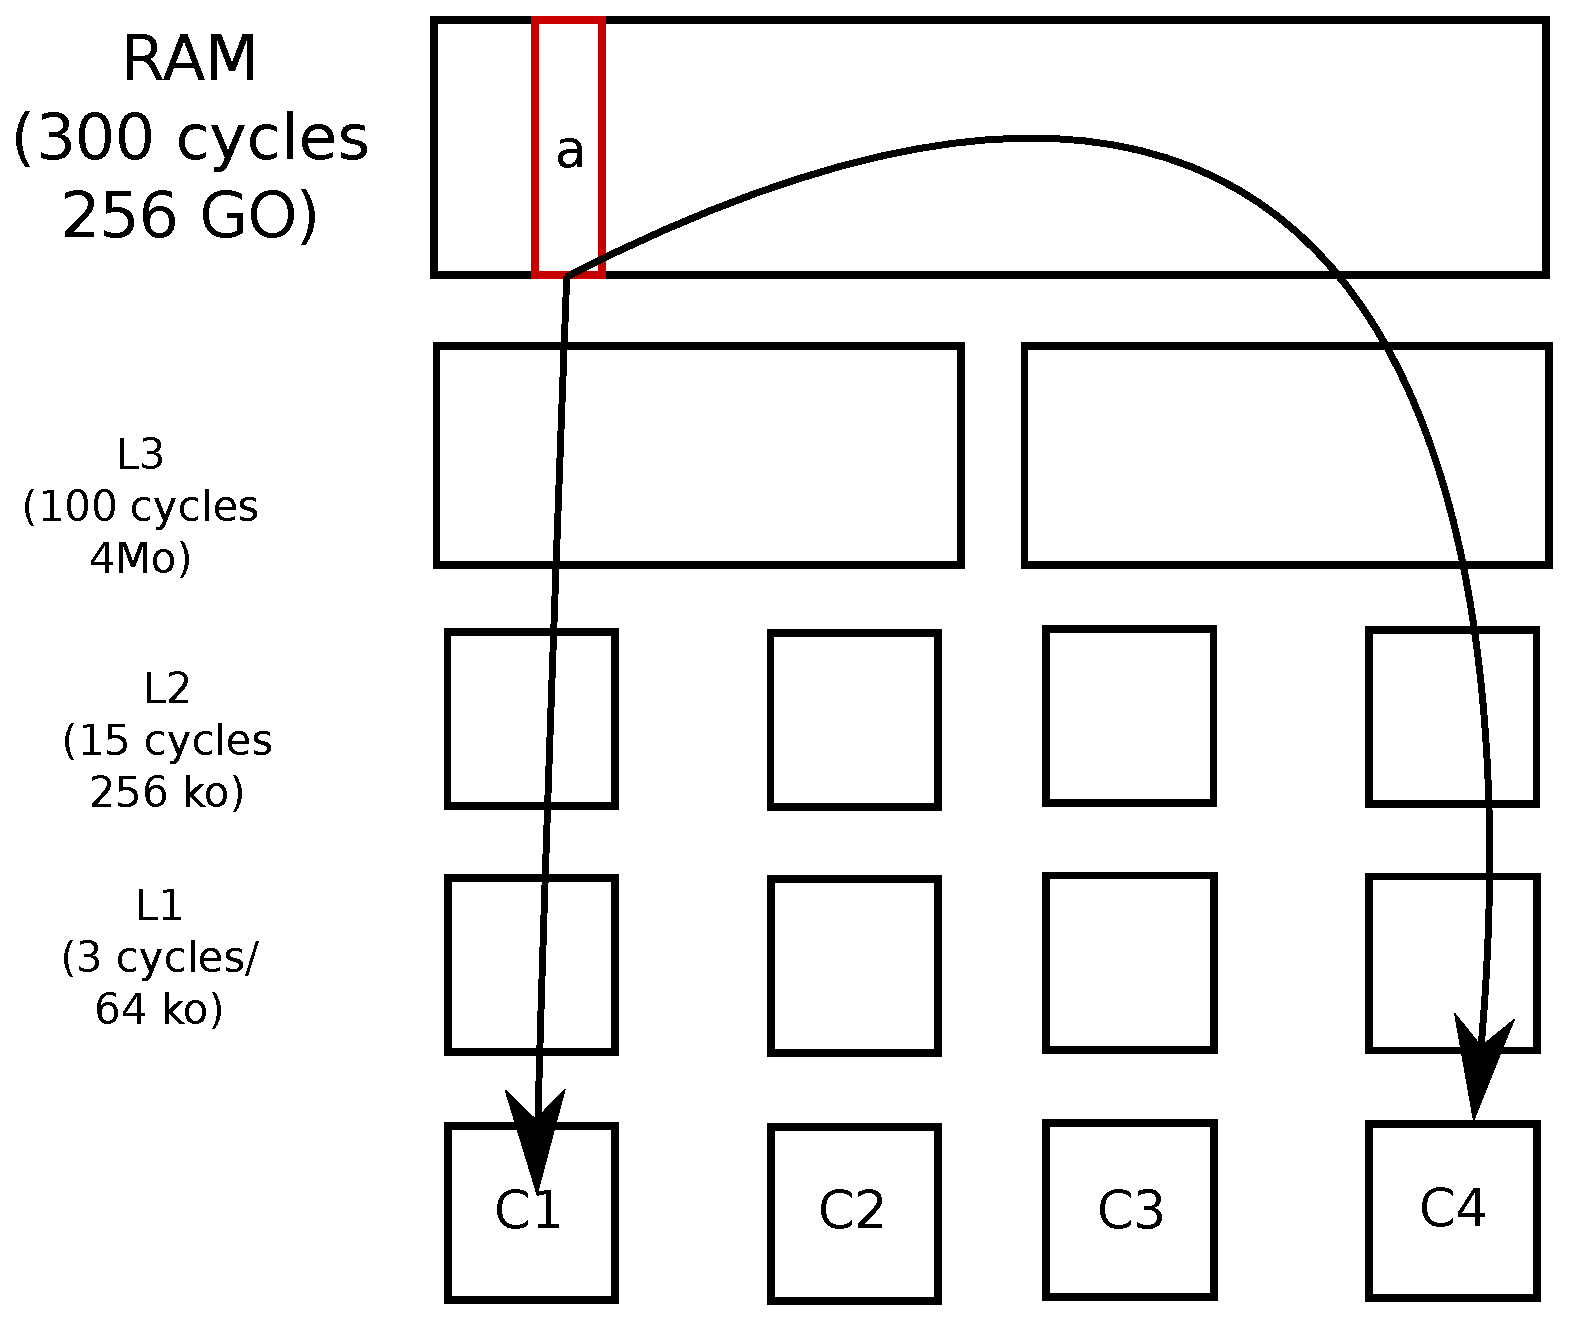
\includegraphics[width=0.5\linewidth]{cache.eps}
\caption{\label{fig:cache}Hiérarchie des caches}
\end{figure}

\paragraph{Problème du cache :}
Il assure la cohérence des données, donne un sens à ce que le processeur voit de la mémoire (cf figure \ref{fig:cache}). Comment invalider une ligne de cache en cas de modification ?

On utilise le processus MOESI : un verrou contenant un état par ligne de cache\footnote{c'est ce problème qui est à l'origine du NUMA}, la synchronisation s'effectuant entre cache de même hiérarchie :
\begin{itemize}
\item[E :] Excusive (Écriture)
\item[I :] Invalid (A été modifiée / plus présente)
\item[S :] Shared (Lecture)
\end{itemize}
Il faut cependant garder l'information "la valeur en cache est-elle plus récente que celle en RAM ?". Pour cela, on dédouble tous les états :
\begin{itemize}
\item[M :] Modified, E mais incohérente avec la mémoire centrale
\item[O :] Owned, S mais incohérente avec la mémoire centrale
\end{itemize}
L'état I n'est pas répliqué puisque la ligne de cache n'a plus aucun sens.
\bigskip

Pour récapituler :
\begin{itemize}
\item[État M ou E :] verrou en écriture
\item[État O ou S :] verrou en lecture
\item[État I :] pas de verrou
\end{itemize}
\bigskip

Où est le soucis ? Avant, on faisait du \emph{snooping} (espionnage) : tout passait par le bus. Le soucis est que le snooping ne scale pas car il demande un \emph{broadcast} (demander à toutes les autres cœurs).

Solution : On segmente la mémoire en centralisant l'accès à certaines lignes de caches qui sont gérés par certains clusters spécifiques. Des tables associent les adresses physiques aux cœurs qui cachent la ligne : ainsi les invalidation seront spécifiquement envoyés au bon processeur. Autre soucis : où mettre la table ? La segmentation se fait en divisant la mémoire par le nombre de cluster et en répartissant équitablement celle ci entre les cluster (noeud 1 $\to$ mémoire de 0 à 2 Go, noeud 2 $\to$ 2 à 4 Go, etc). Le cluster est alors un \emph{nœud NUMA}, qui correspond souvent à un die (bien que ce soit trois dénominations différentes). Le routage s'effectue par chaque nœud NUMA qui connait la table (stockée dans le L3 et gérée par un petit contrôleur), spécifiée pas le BIOS au démarrage.

\paragraph{Note :}
Cette segmentation est nécessaire mais relativement peu utilisée (bcp de variables locales). Dans le meilleur des cas (pas de saturation), une lecture va couter environ 500 cycle. Dans le cas saturé, environ 2000 cycles !

\paragraph{Conséquences :}
L'accès à la mémoire centrale n'est plus uniforme (local : 200 cycles ; au pire, 400 cycles) ; les liens peuvent saturer (et là, 2000 cycles !). La partitionnement de la mémoire change la latence !

\paragraph{Principe/Solution :} augmenter au maximum la localité quand on développe une appli. Par défaut, la mémoire virtuelle est mappée sur différents nœuds NUMA selon la politique \emph{first touch} : si la mémoire n'est pas encore mappée, on lui donne de la mémoire à partir \emph{de son propre noeud}. Dans le cas de gros malloc, le mappage se fait \emph{au niveau des premiers accès} et non au niveau de la réservation.

Il existe également l'\emph{interleaved} qui utilise un \emph{round robin} (allocation aléatoirement de la mémoire), ce qui permet d'équilibrer les accès mais est très mauvais pour la localité (pas de saturation interne).

\subsubsection{Placement de processus sous Linux}
\texttt{pthread\_setaffinity} pour sélectionner le cœur, \texttt{mbind} pour n'allouer la mémoire physique qu'à partir d'un ensemble de nœuds. \texttt{madvise} permet de libérer les pages physiques pour les migrer.



\end{document}